%%	febrero 2018
%%	Autor: Imer A. Robles Rodriguez - imer.robles@correo.uis.edu.co
%%
%%	Archivo que contiene la mayoria de la configuracion complementaria
%%	que no pudo ser agregada en la clase 'icontecUIS.cls'
%%	incluirlo en la primera línea de el archivo.tex de su respectivo libro
%%	%%	febrero 2018
%%	Autor: Imer A. Robles Rodriguez - imer.robles@correo.uis.edu.co
%%
%%	Archivo que contiene la mayoria de la configuracion complementaria
%%	que no pudo ser agregada en la clase 'icontecUIS.cls'
%%	incluirlo en la primera línea de el archivo.tex de su respectivo libro
%%	%%	febrero 2018
%%	Autor: Imer A. Robles Rodriguez - imer.robles@correo.uis.edu.co
%%
%%	Archivo que contiene la mayoria de la configuracion complementaria
%%	que no pudo ser agregada en la clase 'icontecUIS.cls'
%%	incluirlo en la primera línea de el archivo.tex de su respectivo libro
%%	\input{path/to/structure}
%%
%%	Nota 1. en bibstyle=paht/to/icontec-imer, corregir el paht/to/icontec-imer 
%%
%%	Nota 2. para usar la cita icontec se usa el comando \footcite{}, en lugar del típico \cite{}

\documentclass[12pt,oneside,onecolumn,final,openright]{icontecUIS}
\usepackage[utf8]{inputenc}
\usepackage{lmodern}

\usepackage{csquotes}
\usepackage[spanish,es-tabla]{babel}
\usepackage[bibstyle=bib/icontec-imer,citestyle=verbose-trad2,sortcites=true,maxcitenames=3,maxbibnames=9,backend=biber]{biblatex} %


%--------Codigos para la caligrafia, tipos de letras%---------------
\usepackage{textcomp} %Paquete para algunos caracteres especiales
\usepackage[T1]{fontenc}
\usepackage[scaled]{uarial}
%\renewcommand{\familydefault}{\sfdefault} % sans serfi default
\renewcommand{\familydefault}{\rmdefault} % roman default
%\renewcommand{\baselinestretch}{1.5}
\usepackage{setspace}
\usepackage{amsmath,amsfonts}
\usepackage{graphicx}
\usepackage{subfig}
\usepackage{float}
\usepackage{booktabs}

\usepackage{datetime}


\usepackage[pdftex,%unicode=true,%pdftex,
pdfauthor={Imer A. Robles Rodríguez},
pdftitle={Tesis Pregrado},
%pdfsubject={The Subject},
% pdfkeywords={},
pdfproducer={Latex with hyperref, or other system},
pdfcreator={pdflatex, or other tool},
hidelinks,%=true,
bookmarks=true,
linktoc=all]{hyperref}


\usepackage{bookmark}

\usepackage{geometry}
\geometry{
	papersize = {216mm, 279mm}, % tamaño de papel carta colombia
	top = 4cm,
	left = 4cm,
	bottom = 3cm,
	right = 2cm,
	%% configurando notas la margen, encabezado y pie
%	headsep = 0.5em,
%	head = 0em,
	foot = 1cm,
	nomarginpar, nohead,
}


\hyphenation{op-tical net-works semi-conduc-tor}

\usepackage{titlesec}
\titleformat{\section}%[runin]
{\raggedright \normalfont\bfseries\uppercase} %formato
{\thesection.} %label
{0.5em}%separacion horizontal
{} %antes code []% despues code
\titlespacing{\section}{0pt}{*4}{*1}
\titleformat{\subsection}[runin]
{\raggedright \normalfont \bfseries \uppercase} %formato \fontsize{12pt}{12.2pt}
{\thesubsection.}{0.2em}{} %antes code 
[{\newline}]% despues code
\titlespacing{\subsection}{0pt}{*4}{*1}
\titleformat{\subsubsection}[runin]
{\raggedright \large \bfseries} %formato
{\thesubsubsection.} %label
{0.5em}%separacion horizontal
{} %antes code 
%[\vspace{-24pt}]% despues code

%%	comando definido para hacer fácil la inclusión de figuras
%%	\figura{ubicacion-de-figura/imagen}{nombre/caption}{ancho a usar en imagen/tamaño entre 0-1}{fuente/origen de la figura, si es propia dejar vacío}
\newcommand{\figura}[4]{
	\begin{figure}[H]
		\begin{minipage}{\textwidth}
			\caption[#2]{\raggedright #2}
			\label{fig:#2}
			\begin{center}
				\includegraphics[width=#3\textwidth]{#1}\\
			\end{center}
			#4
		\end{minipage}
	\end{figure}
}

\setlength{\parindent}{0em} % sangria (identacion) en 0
\addbibresource{Anexos/LATEX/source/bib/referencias.bib}

\usepackage{lipsum}
\usepackage{float}
\usepackage[utf8]{inputenc}
\usepackage[spanish]{babel}
\usepackage{newunicodechar}
\newunicodechar{fi}{fi}
\newunicodechar{ff}{ff}
%%
%%	Nota 1. en bibstyle=paht/to/icontec-imer, corregir el paht/to/icontec-imer 
%%
%%	Nota 2. para usar la cita icontec se usa el comando \footcite{}, en lugar del típico \cite{}

\documentclass[12pt,oneside,onecolumn,final,openright]{icontecUIS}
\usepackage[utf8]{inputenc}
\usepackage{lmodern}

\usepackage{csquotes}
\usepackage[spanish,es-tabla]{babel}
\usepackage[bibstyle=bib/icontec-imer,citestyle=verbose-trad2,sortcites=true,maxcitenames=3,maxbibnames=9,backend=biber]{biblatex} %


%--------Codigos para la caligrafia, tipos de letras%---------------
\usepackage{textcomp} %Paquete para algunos caracteres especiales
\usepackage[T1]{fontenc}
\usepackage[scaled]{uarial}
%\renewcommand{\familydefault}{\sfdefault} % sans serfi default
\renewcommand{\familydefault}{\rmdefault} % roman default
%\renewcommand{\baselinestretch}{1.5}
\usepackage{setspace}
\usepackage{amsmath,amsfonts}
\usepackage{graphicx}
\usepackage{subfig}
\usepackage{float}
\usepackage{booktabs}

\usepackage{datetime}


\usepackage[pdftex,%unicode=true,%pdftex,
pdfauthor={Imer A. Robles Rodríguez},
pdftitle={Tesis Pregrado},
%pdfsubject={The Subject},
% pdfkeywords={},
pdfproducer={Latex with hyperref, or other system},
pdfcreator={pdflatex, or other tool},
hidelinks,%=true,
bookmarks=true,
linktoc=all]{hyperref}


\usepackage{bookmark}

\usepackage{geometry}
\geometry{
	papersize = {216mm, 279mm}, % tamaño de papel carta colombia
	top = 4cm,
	left = 4cm,
	bottom = 3cm,
	right = 2cm,
	%% configurando notas la margen, encabezado y pie
%	headsep = 0.5em,
%	head = 0em,
	foot = 1cm,
	nomarginpar, nohead,
}


\hyphenation{op-tical net-works semi-conduc-tor}

\usepackage{titlesec}
\titleformat{\section}%[runin]
{\raggedright \normalfont\bfseries\uppercase} %formato
{\thesection.} %label
{0.5em}%separacion horizontal
{} %antes code []% despues code
\titlespacing{\section}{0pt}{*4}{*1}
\titleformat{\subsection}[runin]
{\raggedright \normalfont \bfseries \uppercase} %formato \fontsize{12pt}{12.2pt}
{\thesubsection.}{0.2em}{} %antes code 
[{\newline}]% despues code
\titlespacing{\subsection}{0pt}{*4}{*1}
\titleformat{\subsubsection}[runin]
{\raggedright \large \bfseries} %formato
{\thesubsubsection.} %label
{0.5em}%separacion horizontal
{} %antes code 
%[\vspace{-24pt}]% despues code

%%	comando definido para hacer fácil la inclusión de figuras
%%	\figura{ubicacion-de-figura/imagen}{nombre/caption}{ancho a usar en imagen/tamaño entre 0-1}{fuente/origen de la figura, si es propia dejar vacío}
\newcommand{\figura}[4]{
	\begin{figure}[H]
		\begin{minipage}{\textwidth}
			\caption[#2]{\raggedright #2}
			\label{fig:#2}
			\begin{center}
				\includegraphics[width=#3\textwidth]{#1}\\
			\end{center}
			#4
		\end{minipage}
	\end{figure}
}

\setlength{\parindent}{0em} % sangria (identacion) en 0
\addbibresource{Anexos/LATEX/source/bib/referencias.bib}

\usepackage{lipsum}
\usepackage{float}
\usepackage[utf8]{inputenc}
\usepackage[spanish]{babel}
\usepackage{newunicodechar}
\newunicodechar{fi}{fi}
\newunicodechar{ff}{ff}
%%
%%	Nota 1. en bibstyle=paht/to/icontec-imer, corregir el paht/to/icontec-imer 
%%
%%	Nota 2. para usar la cita icontec se usa el comando \footcite{}, en lugar del típico \cite{}

\documentclass[12pt,oneside,onecolumn,final,openright]{icontecUIS}
\usepackage[utf8]{inputenc}
\usepackage{lmodern}

\usepackage{csquotes}
\usepackage[spanish,es-tabla]{babel}
\usepackage[bibstyle=bib/icontec-imer,citestyle=verbose-trad2,sortcites=true,maxcitenames=3,maxbibnames=9,backend=biber]{biblatex} %


%--------Codigos para la caligrafia, tipos de letras%---------------
\usepackage{textcomp} %Paquete para algunos caracteres especiales
\usepackage[T1]{fontenc}
\usepackage[scaled]{uarial}
%\renewcommand{\familydefault}{\sfdefault} % sans serfi default
\renewcommand{\familydefault}{\rmdefault} % roman default
%\renewcommand{\baselinestretch}{1.5}
\usepackage{setspace}
\usepackage{amsmath,amsfonts}
\usepackage{graphicx}
\usepackage{subfig}
\usepackage{float}
\usepackage{booktabs}

\usepackage{datetime}


\usepackage[pdftex,%unicode=true,%pdftex,
pdfauthor={Imer A. Robles Rodríguez},
pdftitle={Tesis Pregrado},
%pdfsubject={The Subject},
% pdfkeywords={},
pdfproducer={Latex with hyperref, or other system},
pdfcreator={pdflatex, or other tool},
hidelinks,%=true,
bookmarks=true,
linktoc=all]{hyperref}


\usepackage{bookmark}

\usepackage{geometry}
\geometry{
	papersize = {216mm, 279mm}, % tamaño de papel carta colombia
	top = 4cm,
	left = 4cm,
	bottom = 3cm,
	right = 2cm,
	%% configurando notas la margen, encabezado y pie
%	headsep = 0.5em,
%	head = 0em,
	foot = 1cm,
	nomarginpar, nohead,
}


\hyphenation{op-tical net-works semi-conduc-tor}

\usepackage{titlesec}
\titleformat{\section}%[runin]
{\raggedright \normalfont\bfseries\uppercase} %formato
{\thesection.} %label
{0.5em}%separacion horizontal
{} %antes code []% despues code
\titlespacing{\section}{0pt}{*4}{*1}
\titleformat{\subsection}[runin]
{\raggedright \normalfont \bfseries \uppercase} %formato \fontsize{12pt}{12.2pt}
{\thesubsection.}{0.2em}{} %antes code 
[{\newline}]% despues code
\titlespacing{\subsection}{0pt}{*4}{*1}
\titleformat{\subsubsection}[runin]
{\raggedright \large \bfseries} %formato
{\thesubsubsection.} %label
{0.5em}%separacion horizontal
{} %antes code 
%[\vspace{-24pt}]% despues code

%%	comando definido para hacer fácil la inclusión de figuras
%%	\figura{ubicacion-de-figura/imagen}{nombre/caption}{ancho a usar en imagen/tamaño entre 0-1}{fuente/origen de la figura, si es propia dejar vacío}
\newcommand{\figura}[4]{
	\begin{figure}[H]
		\begin{minipage}{\textwidth}
			\caption[#2]{\raggedright #2}
			\label{fig:#2}
			\begin{center}
				\includegraphics[width=#3\textwidth]{#1}\\
			\end{center}
			#4
		\end{minipage}
	\end{figure}
}

\setlength{\parindent}{0em} % sangria (identacion) en 0
\addbibresource{Anexos/LATEX/source/bib/referencias.bib}

\usepackage{lipsum}
\usepackage{float}
\usepackage[utf8]{inputenc}
\usepackage[spanish]{babel}
\usepackage{newunicodechar}
\newunicodechar{fi}{fi}
\newunicodechar{ff}{ff}

% -- Título de la tesis -- %
\title{DESARROLLO DE UN PROTOTIPO DE SOFTWARE COMO SOPORTE A LA REVISIÓN DE PUESTOS LABORALES PARA ANTEBRAZO, MUÑECAS Y MANOS}

% -- Autores -- %
\author{AUTORES:\\\vspace{1cm}\\DANIEL NIETO GÓMEZ\\EMILSON JUNIOR PARRA GAMARRA}

% -- Subtitulo -- %
\legend{ANTEPROYECTO DE GRADO PARA OPTAR POR EL TÍTULO DE INGENIERO DE SISTEMAS}

% -- Director -- %
\director{PAULO ALONSO GAONA GARCÍA}

% -- Título del Director y datos del Codirector -- %
\directortitle{}

% -- Universidad -- %
\institution {UNIVERSIDAD DISTRITAL FRANCISCO JOSÉ DE CALDAS}

% -- Facultad -- %
\faculty {FACULTAD DE INGENIERÍA\\{PROYECTO CURRICULAR INGENIERÍA DE SISTEMAS\\}}

% -- Fecha y Año -- %
\date{Bogotá D.C, 2018}



\begin{document}


%% ---- PREÁMBULO DEL DOCUMENTO ---- %%

% -- Insertar portada y contraportada -- %
\onehalfspace \maketitle

% -- Insertar tabla de contenidos -- %
\tableofcontents

% -- Insertar tabla de figuras -- %
\newpage \listoffigures

% -- Insertar lista de tablas -- %
\newpage \listoftables

% -- Configurar salto de linea -- %
\setlength{\parskip}{\baselineskip} 
\newpage



%% ---- COMIENZO DEL DOCUMENTO ---- %%
	
% -- Capitulo uno: Introducción -- %
\newpage
\chapter{INTRODUCCIÓN} 
La Dirección General de Riesgos Profesionales del Ministerio de la Protección Social publicó en el año 2004 el informe de enfermedades profesionales en Colombia 2001 – 2002, en el cual se define un plan de trabajo cuyo objetivo fundamental es incrementar el diagnóstico y prevenir las enfermedades profesionales de mayor prevalencia en Colombia. Dicho plan de trabajo fue incluido en el Plan Nacional de Salud Ocupacional y Seguridad en el trabajo 2013 – 2021, refrendando de esta manera el compromiso del Ministerio frente al tema de la prevención de las enfermedades profesionales.

Si bien los desórdenes músculo esqueléticos relacionados con el trabajo (DME) son entidades comunes y potencialmente discapacitantes, son prevenibles, por tal motivo, fue creada la Guía de Atención Integral de Salud Ocupacional (GATISO) basada en la evidencia para Desórdenes Músculo Esqueléticos (DME) relacionados con movimientos repetitivos de miembros superiores. A pesar de que la guía fue elaborada para prevenir, realizar el diagnóstico precoz y proporcionar tratamiento a los trabajadores en riesgo de sufrir o ser afectados por las enfermedades más comunes, el riesgo de sufrir una lesión de esta categoría sigue latente debido a que el periodo de tiempo sobre el cual se realiza la evaluación es muy reducido.

Si bien a durante los últimos años se han desarrollado herramientas para automatizar el proceso como lo es \textit{'ILENA'}\footnote{Herramienta computacional en donde por medio del dispositivo Kinect se determinan falencias en los movimientos a partir de las posiciones ergonómicas esperadas} propuesta por \parencite{Moya2015ModeloOcupacional}, se vuelve notable la inexactitud al momento de evaluar los miembros distales superiores\footnote{Manos, muñeca y antebrazo} ya que el sensor carece de precisión, de esta manera descuidando la zona donde se focalizan la mayoría de los desórdenes músculo esqueléticos padecidos, en particular, por personas que desempeñan labores de computo.

Por ende resultaría interesante contar la implementación un dispositivo que pueda ser utilizado en la oficina y permita monitorear y detectar movimientos ergonómicamente incorrectos realizados con los miembros distales superiores con el fin de incrementar el diagnóstico y prevenir las enfermedades profesionales de oficina de mayor predominio en Colombia y así fortalecer las herramientas disponibles para contrarrestar la problemática.

Partiendo de esta necesidad, se plantea el proyecto presente en busca de crear nuevas soluciones para la salud ocupacional, teniendo como objetivo diseñar y construir una solución que integre dispositivos de hardware existentes con software basado en inteligencia artificial que permita dar soporte a los procesos de monitoreo del puesto de trabajo, para la evaluación o estudio del mismo, lo anterior siendo fundamentado sobre tecnologías de desarrollo libre.

% -- Capitulo dos: Problema De Investigación -- %
\chapter{PROBLEMA DE INVESTIGACIÓN}

\section{DESCRIPCIÓN DEL PROBLEMA}
Las instituciones de salud ocupacional son las encargadas de realizar los procesos de evaluación de puestos laborales, estos procesos permiten a las empresas contar con información de calidad para evitar trastornos ergonómicos que puedan perjudicar la salud de los trabajadores, sin embargo, estos procesos no son perfectos y se encuentran en constante optimización para incrementar los niveles de fiabilidad. Por tal motivo se busca fortalecer los procesos de salud ocupacional, pretendiendo garantizar que el entorno de trabajo se encuentre en armonía con las actividades que realiza el trabajador. %, lo anterior se refleja en la productividad, la calidad, la seguridad, la salud, la fiabilidad, la satisfacción con el trabajo y en el desarrollo personal de los trabajadores.\footcite[3]{MiguelAGonzalezPerez}

Actualmente se examinan las condiciones de los puestos de trabajo desde una perspectiva ergonómica con el propósito de obtener una detección temprana de condiciones o actos subestándar y finalmente culminar en los controles necesarios para disminuir la probabilidad de presentar alteraciones osteomusculares, desórdenes músculo esqueléticos o enfermedades laborales relacionadas. Sin embargo, estas revisiones solo se ejecutan en un intervalo de tiempo determinado durante el cual la persona que está siendo evaluada asume las posiciones correctas al sentirse observada e impide un diagnóstico efectivo de vicios posturales, además, las herramientas tecnológicas dispuestas para automatizar este proceso se encuentran diseñadas con sensores RGB-D que evalúan todo el cuerpo, dejando de lado la precisión requerida para analizar los desórdenes músculo esqueléticos de la mano, muñeca y antebrazo

Lo descrito anteriormente, repercute en demoras para realizar los cambios en cuanto al mejoramiento en las condiciones y adaptación de los puestos de trabajo. Por tal motivo, se busca implementar una estrategia que permita tener un método de observación objetivo que perciba, identifique y puntualice los vicios posturales. Esto contribuiría a la exactitud y neutralidad al realizar una inspección de puesto laboral.

La empresa Latino BI Consulting presenta antecedentes de los síntomas descritos previamente en sus trabajadores, con lo cual, se convierte en una unidad de análisis sobre la cual implementar los métodos propuestos y analizar el proceso, el desarrollo y los resultados obtenidos que merecen atención en el futuro.

Por lo tanto se decide poner en marcha el proyecto ‘NOMBRE DEL PROYECTO’ en su primera versión, en donde se propone diseñar, desarrollar y probar un prototipo de software como soporte a la gestión de la revisión de puestos de trabajo para los miembros superiores al utilizar un mouse y teclado.

\section{FORMULACIÓN DEL PROBLEMA}
De acuerdo a la problemática descrita anteriormente, se plantea la siguiente pregunta que guiará el desarrollo de la propuesta de trabajo ¿Cómo desarrollar un prototipo de software que facilite el proceso de revisión de puestos de trabajo en una organización?

% -- Capitulo tres: Objetivos -- %
\chapter{OBJETIVOS}
\section{OBJETIVO GENERAL}
\paragraph{Propuesta 1}
Desarrollar un prototipo de software que permita apoyar el proceso de revisión de puestos de trabajo a partir de una evaluación ergonómica constante sobre la postura de los miembros superiores durante las actividades laborales.
\paragraph{Propuesta 2}
Crear a partir de una herramienta de hardware un prototipo de software, que permita a través de una interfaz de lenguaje natural, capturar los movimientos de las extremidades superiores en puestos de trabajo, que permita tener una evaluación dinámica y  constante de la pulcritud postural durante toda la ejecución de la actividad laboral. 
\section{OBJETIVOS ESPECÍFICOS}
\begin{itemize}
    \item Determinar las condiciones ergonómicas adecuadas para las muñecas y antebrazos a partir de una revisión sistemática de los estándares utilizados por especialistas de salud ocupacional en el contexto nacional e internacional para determinar vicios posturales,  de esta manera precisando el modelo que más se adecúa al prototipo propuesto.
    \item Diseñar un modelo computacional para la interpretación de los datos generados por la herramienta de hardware LeapMotion.
    \item Adoptar una metodología que permita desarrollar de forma ágil un prototipo de software que evalúe la postura del antebrazo y mano en tiempo real. 
    \item Establecer un modelo de evaluación para los datos capturados por la herramienta que determine las posturas ergonómicamente incorrectas. 
\end{itemize}

% -- Capitulo cuatro: Justificación -- %
\chapter{JUSTIFICACIÓN}
En los últimos 10 años se ha evidenciado un importante crecimiento en el uso de computadores como elemento de trabajo principal en las oficinas, asimismo, el DANE (Departamento Administrativo Nacional de Estadística)  muestra que 99.4\% de las empresas en los sectores de industria manufacturera, comercio y servicios poseen al menos un computador y de este total general el 75.83 \% usan el computador de forma diaria durante aproximadamente 6 horas de las 8 horas laborales establecidas.\footcite[]{Dane2013IndicadoresEmpresas}

A pesar de que las empresas Administradoras de Riesgos Laborales (ARL) realizan revisiones de puestos de trabajo, el Informe Colombiano de Enfermedades Profesionales para el 2017 indica que la tasa de enfermedades laborales para el país fue de 94,7 por cada 100.000 trabajadores, (FASECOLDA). Teniéndose de esta manera, uno de los aspectos más importantes que justifican el proyecto 'NOMBREDELPROYECTO', el cual gira entorno a la reducción de Desórdenes Músculo Esqueléticos (DME) a causa de exigencias biomecánicas no supervisadas en los puestos de trabajo.



% Añadir justificación desde:
% 1. Perspectiva Monetaria: Las empresas pierden plata
% 2. Enfoque humano: Las personas quedan lesionadas PERMANENTEMENTE teniendo menor calidad de vida
% 3. Gastos en Salud: El estado gasta X plata cubriendo DME

por esa razón se pretende estudiar los factores de riesgo laboral que influyen en el desarrollo de este tipo de lesiones del tren superior y extremidades, y la influencia de los factores del trabajo como determinados movimientos repetitivos y posturas


% -- Capitulo cinco: Marco Teórico -- %
\chapter{MARCO TEÓRICO}
\section{MARCO CONCEPTUAL}
\subsection{LeapMotion}
.
\subsection{Goniometria}
.
\subsection{Análisis de puesto de trabajo}
.
\subsection{Enfermedades y lesiones}
 Un Desorden Músculo Esquelético (DME) es una lesión física originada por trauma acumulado que se desarrolla gradualmente sobre un período de tiempo; como resultado de repetidos esfuerzos sobre una parte específica del sistema músculo esquelético. \footcite[]{MinisterioQue}. A continuación se presentan las enfermedades prevalentes en los puestos de trabajo para manos, muñeca y antebrazo

\subsubsection{Tenosinovitis De Quervain}
\paragraph{¿Qué es?}
La Tenosinovitis De Quervainn (TDQ) también conocida como tenosinovitis estiloides radiales, consiste en la inflamación de los tendones del pulgar a causa de movimientos repetitivos.

\begin{figure}[H]
    \centering
    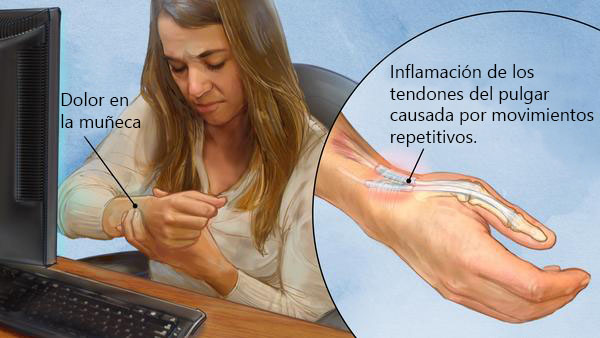
\includegraphics[width=0.7\textwidth]{Anexos/LATEX/chapters/images/TDQ.jpg}
    \caption{Anatomía de la mano con TDQ \\\textbf{Fuente:} https://g.co/kgs/BpkB4A}
    \label{TDQ}
\end{figure}

Esta enfermedad se manifiesta como una inflamación que produce una estenosis del canal osteofibrososinovial situado en la estiloides radial por el que discurren los tendones del abductor largo y extensor corto del pulgar. Se produce al combinar agarres con giros o desviaciones cubitales y radiales repetidas o forzadas de la mano.\footcite[2]{TenosinovitisDelPulgarDDCENFERMEDADESTME}

De acuerdo al Instituto Nacional de Seguridad e Higiene en el Trabajo de España, la Enfermedad de Quervain (CIE-9 MC 727.04) posee un tiempo estándar de incapacidad temporal de 20 días.\footcite[6]{TenosinovitisDelPulgarDDCENFERMEDADESTME}
\paragraph{Prevención}
Se aconseja no combinar agarres con giros o desviaciones cubitales y radiales repetidas. Para las situaciones de oficina que involucran un mouse, es necesario evitar realizar desplazamientos girando la muñeca, el movimiento adecuado debe ser desplazar el brazo en su totalidad desde el hombro
\subsubsection{Síndrome del Túnel del Carpo}
\paragraph{¿Qué es?}
Existe un espacio en la muñeca llamado túnel del carpo, a través del cual pasan el nervio mediano y nueve tendones flexores que van desde el antebrazo hacia la mano. El Síndrome del Túnel del Carpo (STC) es una condición producida por la compresión del Nervio Mediano, a nivel de la muñeca. Esta compresión produce entumecimiento, hormigueo y dolor en la mano, dedos y ocasionalmente en el brazo. \footcite{SindromeCarpiano}

\begin{figure}[H]
    \centering
    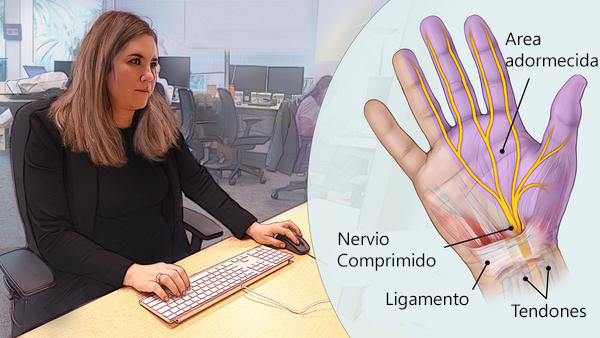
\includegraphics[width=0.7\textwidth]{Anexos/LATEX/chapters/images/STC.jpg}
    \caption{Anatomía de la mano con STC \\\textbf{Fuente:} https://g.co/kgs/MdPBTe}
    \label{STC}
\end{figure}

El STC se presenta cuando se aumenta la presión dentro del túnel por cualquier proceso inflamatorio, comprimiendo el nervio, el cual es una estructura muy sensible a los aumentos de presión. Cuando la presión dentro del túnel es muy alta y altera la función normal del nervio, aparecen rigidez, hormigueo y dolor en la mano y los dedos.\footcite{SindromeCarpiano}
\paragraph{Prevención}
Es recomendable informar al trabajador, entrenándolo para que aquellas posturas o movimientos peligrosos sean evitados durante el desarrollo de su labor, además, el buen diseño de las herramientas, utensilios y del puesto de trabajo ayudan a conseguir la relajación de la mano y de la muñeca.\footcite{SindromeTratarlo}

\subsubsection{Síndrome del túnel cubital}
%http://www.insht.es/InshtWeb/Contenidos/Documentacion/FICHAS%20DE%20PUBLICACIONES/EN%20CATALOGO/ERGONOMIA/Ficha6epitrocleoolecranian.pdf
\subsection{Legislación Vigente}
\section{MARCO REFERENCIAL}
\subsection{Modelos de valoración del riesgo contexto nacional}
\subsubsection{Normas GATI-SO}
Las Guías de Atención Integral de Salud Ocupacional Basadas en la Evidencia (GATI-SO) nacen a partir de un plan de trabajo propuesto por la dirección general de riesgos profesionales del ministerio de la protección social con el objetivo de incrementar el diagnóstico y prevenir las enfermedades profesionales de
mayor prevalencia en Colombia.\footcite[6]{MinisterioQue}

Las características de los factores de riesgo ocupacional que han demostrado estar asociados con la aparición del \textbf{STC} son las siguientes:\footcite[45]{MinisterioQue}
\begin{itemize}
\item Posturas en flexión y extensión de dedos, mano y muñeca, así como, la desviación ulnar o radial que implique agarre, pronación y supinación combinada con el movimiento repetitivo en ciclos de trabajo
\item Fuerza ejercida en trabajo dinámico por manipulación de pesos en extensión y flexión de los dedos y la mano
\item Vibración segmentaría derivada del uso de herramientas vibratorias
\end{itemize}
Las características de los factores de riesgo ocupacional que han demostrado estar asociados con la aparición del \textbf{TDQ} son las siguientes:\footcite[45]{MinisterioQue}
\begin{itemize}
\item Postura forzada de muñeca asociada a movimiento de alta repetición (ciclos de tiempo menores a 30 segundos o 50 \% del ciclo gastado.
\end{itemize}
Adicionalmente se mencionan las siguientes conclusiones:\footcite[46]{MinisterioQue}
\begin{itemize}
\item Existe evidencia de que las posturas asumidas de codo, antebrazo y mano se asocian con mayor frecuencia a los desórdenes de trauma acumulativo en población trabajadora.
\item Existe evidencia de que el movimiento repetitivo se asocia con mayor frecuencia a los desórdenes de trauma acumulativo en población trabajadora.
\item Existe evidencia de que la fuerza se asocia con mayor frecuencia a los desórdenes de trauma acumulativo en población trabajadora.
\end{itemize}



\section{Métodos de evaluación de posturas}
El factor de riesgo que más se relaciona a la aparición de DME se conoce como carga postural. Cuando se llevan a cabo posturas inadecuadas a manera continua o repetitiva se genera fatiga, la cual con el tiempo puede ocasionar problemas de salud. Por lo tanto, la medición de la carga postural constituye el pilar principal en el proceso de mejora de puestos de trabajo.\footcite[144]{RamosEdgarShrawan2004WorkingReview}
\subsection{Método Rula}
El método RULA tiene como objetivo de evaluar la exposición de los trabajadores a factores de riesgo que originan una elevada carga postural y que pueden ocasionar trastornos en los miembros superiores del cuerpo. Para la evaluación del riesgo se consideran el método la postura adoptada, la duración, la frecuencia y las fuerzas ejercidas cuando se mantiene.\footcite[2]{McatamneyRULA:Disorders}

Para una determinada postura RULA obtendrá una puntuación a partir de la cual se establece un determinado Nivel de Actuación. El Nivel de Actuación indicará si la postura es aceptable o en qué medida son necesarios cambios o rediseños en el puesto. En definitiva, RULA permite al evaluador detectar posibles problemas ergonómicos derivados de una excesiva carga postural.\footcite{Diego-Mas2015EvaluacionRULA}.

RULA divide el cuerpo en dos grupos, el Grupo A que incluye los miembros superiores (brazos, antebrazos y muñecas) y el Grupo B, que comprende las piernas, el tronco y el cuello. Mediante las tablas asociadas al método, se asigna una puntuación a cada zona corporal (piernas, muñecas, brazos, tronco...) para, en función de dichas puntuaciones, asignar valores globales a cada uno de los grupos A y B
\subsection{Método Reba}
\subsection{Método Owas}
\subsection{Evaluación Postural Rápida}
\subsubsection{}
\section{MARCO TECNOLÓGICO}

% -- Capitulo seis: Alcances y Limitaciones -- %
\chapter{DELIMITACIÓN}
\section{ALCANCES}
El presente proyecto contempla la realización de un prototipo de software de escritorio basado en inteligencia artificial, que tiene como finalidad dar soporte al proceso de revisión de puestos de trabajo a partir de una evaluación ergonómica de los miembros distales superiores y enfocado en particular a personas que se desempeñan labores de computo, lo anterior llevado a cabo a través de la captura, análisis y clasificación de los datos generados por la herramienta de hardware, concluyendo en la asignación de una calificación que representa el factor de riesgo asociado a las lecturas percibidas.

\section{LIMITACIONES}
\begin{itemize}
\item El análisis será ejecutado sobre los miembros distales superiores (Mano, muñeca y antebrazo)
\item El sistema no diagnosticará desordenes musculo esqueléticos presentes.
\item La herramienta no estará diseñada para proporcionar procesos de rehabilitación o terapias ni para remitir automáticamente los resultados a una dependencia específica.
\end{itemize}

% -- Capitulo siete: Metodología -- %
\chapter{METODOLOGÍA}

El tipo de investigación realizada es de enfoque experimental, este tipo de investigación consiste en la manipulación directa de una variable independiente, la comparación de dos o mas grupos de condiciones, la medición de cada variable de forma dependiente y un diseño con estadística inferencial que permita el control máximo de variables extrañas.\parencite{MoroneMetodosCientifica}

El proyecto estará dividido en tres fases organizadas y estructuradas para abarcar la totalidad del mismo de forma ágil y efectiva, estas son, fase de análisis, fase de diseño y construcción, y fase de evaluación o validación del producto.

A continuación, se realiza una descripción de cada una de ellas, comenzando en la fase de análisis 
\begin{itemize}
\item Elaboración de entrevistas con profesionales en Salud y seguridad en el trabajo (SST), Salud ocupacional y medicina, como herramienta de investigación se realizará el cuestionario clave para entrevistas a profesionales en el área a SST.
\item Aplicación de entrevistas a profesionales en Salud y seguridad en el trabajo (SST), Salud ocupacional y medicina.
\item Revisión bibliográfica, Se realizará una investigación documental, para condensar el volumen de información relacionada procedente de diferentes fuentes que permitan realizar una comparación de diferentes posturas frente a el tema y sintetizar las ideas en el proyecto. 
\item Consolidación del modelo de valoración de riesgo postural, a partir de la información recolectada de los profesionales y los referentes nacionales e internacionales se realiza un modelo que desde la ergonomía identifique hasta donde un movimiento con cierta repetividad y ángulo se convierte en un riesgo. 
\item Afianzamiento de parámetros de entrada, se definen los posibles parámetros de entrada del sistema.
\item Exploración de técnicas con IA para clasificación, la selección de la herramienta de IA es importante para correcta ejecución del proyecto, por lo tanto, se realizará una exploración de las técnicas posibles que responden al problema de clasificación identificado. 

\end{itemize}

La siguiente fase está denominada como fase de diseño y construcción, la cual está dividida en la siguientes sub-fases.
\begin{itemize}
\item Diseño del modelo arquitectural, Se realiza el diseño arquitectural del prototipo de software, contemplando la estructura entre los elementos y las relaciones de estos.
\item Validación del modelo arquitectural, Es un proceso en el que se validará el nivel de abstracción del modelo y verificación de la correctitud técnica, esto permitirá asegurar la integridad técnica del prototipo a construir.  
\item Diseño modulo preparación de datos (recolección y tratamiento), Se definirá el proceso de organización y normalización de los datos recolectados para tratamiento.
\item Selección de técnica de IA para clasificación, se determinará cual algoritmo de machine learning se ajusta mejor al problema.
\item Diseño de módulo de interpretación, se identificarán las características que tendrá el modelo de IA, incluyendo el ajuste de los parámetros.
\item Construcción de la herramienta, La herramienta está enmarcada en la metodología ágil SCRUM, posteriormente, dependiendo del modelo arquitectural se definirá la lógica de negocio.

\end{itemize}

Para terminar se realizará la fase de validación en la que se realizará un comprobación de la herramienta contra los resultados teóricos, además se realizarán pruebas piloto supervisadas por profesionales en Salud y seguridad en el trabajo (SST), Salud ocupacional y medicina con la finalidad de obtener las respectivas validaciones y afinar el modelo, para culminar, se realizará la compilación de la documentación y entrega.


\subsection{Metodología de software (SCRUM)}
Las metodologías de software ordenan y promueven buenas prácticas en el desarrollo de software de calidad, actualmente se encuentran numerosos modelos y metodologías que se pueden adaptar dependiendo las necesidades del producto final a entregar\parencite{Nohemy2015ESCOGERDECISION}. Para el proyecto ErgoSent se identificaron dos perspectivas importantes que orientan la selección de la metodología, inicialmente debe permitir el desarrollo en un marco de tiempo corto; para este proyecto en específico de 6 meses y por otra parte necesita una verificación diaria con participación constante de expertos, permitiendo un crecimiento preciso y controlado, en donde se tomen decisiones rápidas y adaptables acorde al desarrollo de la aplicación.


Antes de comenzar es necesario definir el producto, el equipo de SCRUM y las tareas generales a realizar, para así elaborar la estructura del proyecto con la metodología, el equipo de trabajo estará compuesto así: 
\begin{itemize}
    \item Product Owner:  Con el objetivo de tener varios puntos de vista, hemos conseguido un grupo de profesionales que nos permiten tener una visión interdisciplinar para cumplirán este rol.
    \begin{enumerate}
        \item Diana Rivera Castillo, Ingeniera industrial con especialización en salud ocupacional, Youtuber Colombiana más influyente en Salud y seguridad en el trabajo SST, y actual Gerente de HSEQ Nueva Visión.
        \item Jorge Enrique Moreno Collazos, Fisioterapeuta, especialista en rehabilitación Cardiopulmonar, magíster en ciencias de la actividad física y el deporte, magíster en calidad educativa, doctor en salud pública, doctor en terapia manual, doctor en educación, Pos doctorado en educación, ciencias sociales e interculturalidad. Docente e investigador.
        \item Ximena Cano, Médica de la Universidad de Ciencias Aplicadas y Ambientales U.D.C.A. 
    \end{enumerate}

\item Scrum Master: esté cargo estará ocupado por Daniel Nieto Gomez.
\item Equipo desarrollador: Estará compuesto por Junior Parra como desarrollador de Scripting en Back end C\# y análisis de software, junto con Daniel Nieto Gómez como diseñador y desarrollador Front end y Análisis enfocado en el uso de herramientas de IA (inteligencia artificial). 
\end{itemize}

La duración del Sprint será de 2 semanas, por el periodo correspondiente al proyecto, es decir, 6 meses.

Por tratarse de un producto de software, la primera tarea a llevar a cabo es la ingeniería o levantamiento de requerimientos, identificando los casos de uso más importantes y requisitos de alto nivel, discutiéndolos con los product owners y  partes interesadas, posteriormente, se escriben en el SCRUM product Backlog y se da inicio a la estimación y priorización de las sesiones con el equipo SCRUM, Luego se comienzan a dividir los requerimientos de alto nivel en requerimientos más pequeños, que se puedan enmarcar en historias de usuario, una vez realizada esta tarea, se convoca a la reunión de planeación del primer Sprint (Sprint planning meetting).

\begin{figure}[H]
    \centering    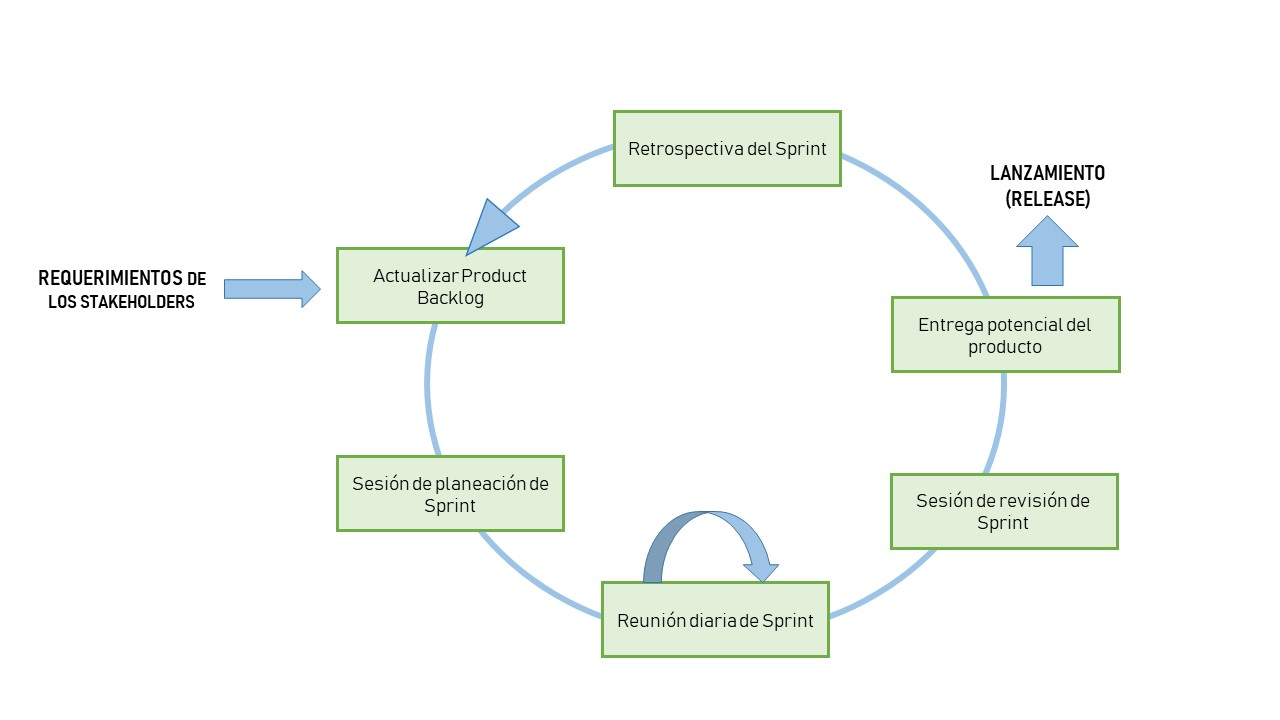
\includegraphics[width=1\textwidth]{Anexos/LATEX/chapters/images/Scrum_1.jpg}
    \caption{Diagrama de Fases y Sprints para el proyecto}
    \small{\textbf{Fuente:} Elaboración propia}
    \label{SCRUM2}
\end{figure}

Con la finalidad de dar soporte a los sprint diarios, se utilizará la plataforma de desarrollo colaborativo Github, facilitando el alojamiento del proyecto y obteniendo control sobre el versionamiento.








% -- Capítulos sin definir -- %
\chapter{RECURSOS}
\chapter{PRESUPUESTO}
\chapter{CRONOGRAMA}

% -- Bibliografía -- %
\newpage
\printbibliography[heading=bibintoc,title={BIBLIOGRAFÍA}]
    
\end{document}